% !TEX root = ../main.tex
\ulfgchapter{4}{Detectors and Evaluation Protocol}{chp:detectors}

\section{Introduction}

This chapter specifies the two detectors compared in this report and fixes the rules by which they
are scored. Choosing an evaluation protocol after seeing comparative results risks introducing
bias, so the protocol is fixed before the benchmark result is examined.

The chapter is organised around the fairness problem set out in Section~\ref{sec:problem}. Each of
the asymmetries listed there is addressed by a specific choice recorded here: the network's
receptive field is matched to the CFAR window; both detectors are reduced to the same output type
and scored by one code path; operating points are matched at measured rather than design
false-alarm rate; and results are reported at more than one matching tolerance.

\subsection*{What is held in common, and what is not}
\label{sec:whatiscommon}

It is worth being exact about this at the outset, because the fairness of the comparison rests on
it and it is easy to overstate.

Both arms are detector arms that turn the same range--Doppler map into a per-cell score map, and
both score maps are then handled identically. What they share is:

\begin{itemize}
\itemsep2pt
\item the \textbf{same underlying range--Doppler data} --- the identical frames, from the identical
processing chain of Chapter~\ref{chp:simulator};
\item a \textbf{comparable local spatial footprint}, $\CfarWinR \times \CfarWinD$ cells, by
construction;
\item the \textbf{same downstream evaluation} --- one peak extractor, one matcher, one set of
metrics, one code path.
\end{itemize}

What they do \emph{not} share is the transform applied between the map and the score. CFAR operates
on range--Doppler power and forms a local ratio statistic. TinyCNN applies a fixed logarithmic
normalisation relative to the frame median before inference, described in
Section~\ref{sec:inputrep}. \textbf{Their input processing is therefore not mathematically
identical}, and this report does not claim it is. Each arm has a fixed, detector-specific transform
that is part of what that detector \emph{is}: a CFAR detector without its ratio is not CFAR, and a
network evaluated on a different normalisation from the one it was trained on is not the trained
network.

The controlled variable is therefore the local decision rule, with as many other factors held
common as is practical --- not every factor, and the exceptions are stated where they arise.

\section{The classical arm}

\subsection{Window geometry}

CFAR requires a reference window, and its shape is a design choice. The window used throughout this
report spans \CfarWinR{} bins in range by \CfarWinD{} in Doppler. Of its \CfarWinCells{} cells,
\textbf{1} is the cell under test, \textbf{\CfarNGuard{}} are guard cells excluded from the
estimate, and \textbf{\CfarNRef{}} are reference cells forming the background estimate $Z$.
Figure~\ref{fig:window} shows the layout.

\begin{figure}[H]
\centering
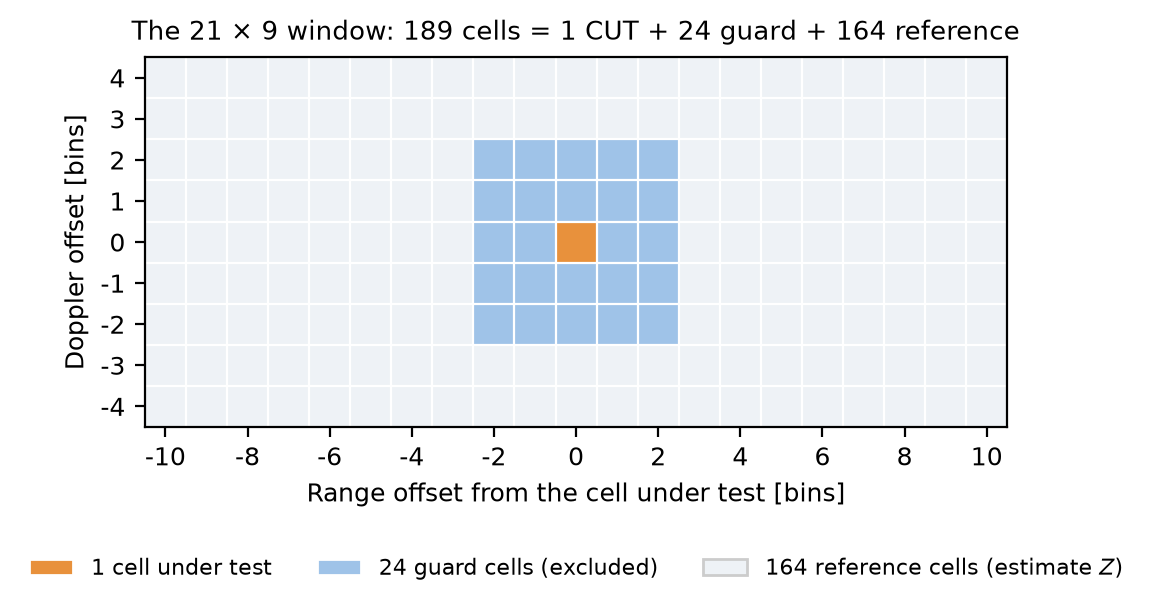
\includegraphics[width=0.95\textwidth]{figures/Chapter4/ch4_fig1_window.png}
\caption[The CFAR reference window used]{The reference window used by every CFAR arm in this
report. Counting outward from the centre, the range axis has \CfarGuardR{} guard cells then
\CfarTrainR{} reference cells on each side; the Doppler axis has \CfarGuardD{} and \CfarTrainD{}.}
\label{fig:window}
\end{figure}

Two aspects of that geometry were decided by measurement rather than convention.

\textbf{The guard count follows the measured point spread function.} Chapter~\ref{chp:simulator}
measured a mainlobe spanning about two bins. The guard ring must cover a target's own spread, or
the target inflates its own threshold and suppresses itself, so \CfarGuardR{} guard cells per side
is the smallest value that does the job.

\textbf{The window is rectangular because the two axes are not alike.} The range axis has
\RadarRangeBins{} bins and no large-scale structure; the Doppler axis has only \RadarM{} and
carries the zero-Doppler clutter ridge. A window sized for range would span a third of the Doppler
axis and drag ridge energy across a wide band of thresholds. Figure~\ref{fig:geomsweep} shows the
candidate geometries evaluated on the dedicated tuning split.

\begin{figure}[H]
\centering
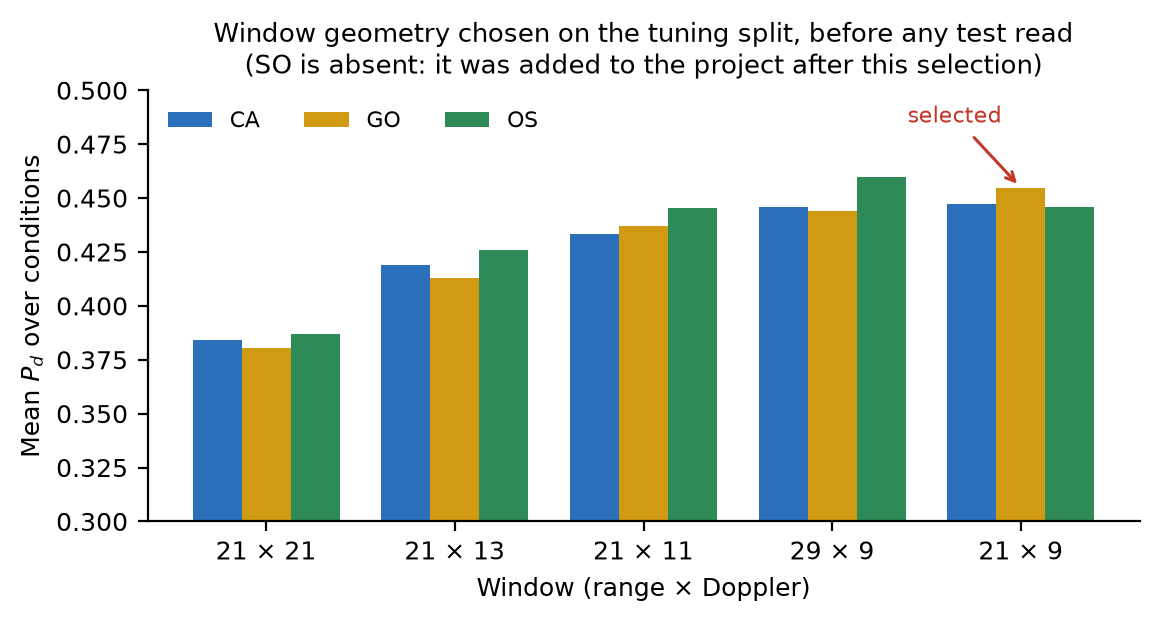
\includegraphics[width=0.88\textwidth]{figures/Chapter4/ch4_fig3_geometry_sweep.png}
\caption[Window geometry selection]{Mean detection probability across conditions for each candidate
window, measured on \texttt{bench2\_tune}. The selected geometry was fixed before any read of the
test split. Only CA, GO and OS appear, for the reason given below.}
\label{fig:geomsweep}
\end{figure}

The selection was made on \texttt{bench2\_tune}, a split used for nothing else. This matters
because the network's operating point is selected on \texttt{bench2\_val}: if both selections used
the same data, one arm would effectively be tuned on the other's selection set.

\textbf{SO-CFAR did not take part in this selection.} SO was added to the project after the window
geometry had already been chosen, and the geometry sweep was never re-run to include it. SO
therefore inherits a window selected on the evidence of the other three variants rather than one
chosen with SO in mind. This is stated rather than repaired: re-running the sweep would change a
selection made before the frozen results were produced, and the honest course is to record that SO
is the one variant whose window was not selected on its own behalf. If SO is disadvantaged by the
choice, that disadvantage is a property of this evaluation and not of the algorithm.

\subsection{Variants}

Four variants are evaluated, differing only in how the reference cells become $Z$: CA, GO, SO and
OS, as described in Section~\ref{sec:cfar_failures}. OS uses a rank fraction of \CfarOsRank{}.
That fraction was never swept, which is a stated limitation: a better-tuned OS might do better than
the one reported here.

\subsection{Threshold calibration}
\label{sec:alphacal}

Two distinct calibrations occur in this report, at different stages and for different purposes.
They are easy to confuse, so they are separated here before either is described.

\begin{description}
\itemsep3pt
\item[(A) Threshold-multiplier calibration.] Described in this section. It fixes a baseline
multiplier $\alpha$ for each CFAR variant, using \emph{noise-only} data. It concerns the CFAR
statistic alone, before any comparison with the network, and it is what Table~\ref{tab:alphas}
reports.
\item[(B) Operating-point matching.] Described in Section~\ref{sec:opoint}. This is the headline
comparison. Each detector's \emph{score threshold} is swept and the two arms are compared at the
same \emph{measured} false-alarm rate. It happens after the shared peak-extraction path, and it
applies to both arms.
\end{description}

\textbf{Table~\ref{tab:alphas} is not the headline comparison.} It reports (A). The reported $\Pd$
values in Chapter~\ref{chp:synthetic} come from (B), where thresholds are swept rather than taken
from the table.

Turning to (A): the multiplier that achieves a chosen false-alarm rate has a closed form for
CA-CFAR, given as equation~\eqref{eq:alpha_ca}. It is not used, for reasons the measurements below
make plain.

All four multipliers are instead obtained by Monte-Carlo calibration. Pure-noise frames are passed
through the identical processing chain, the CFAR ratio map is computed for each, the ratio values
are pooled over all validly tested cells, and the multiplier is taken as the $(1 - \Pfa)$ empirical
quantile of that pooled distribution. The result is the level exceeded by exactly a fraction $\Pfa$
of noise cells, by construction, and it requires no distributional assumption --- which matters,
because only CA has a tractable one.

Figure~\ref{fig:alphacal} shows the calibration and what it corrects.

\begin{figure}[H]
\centering
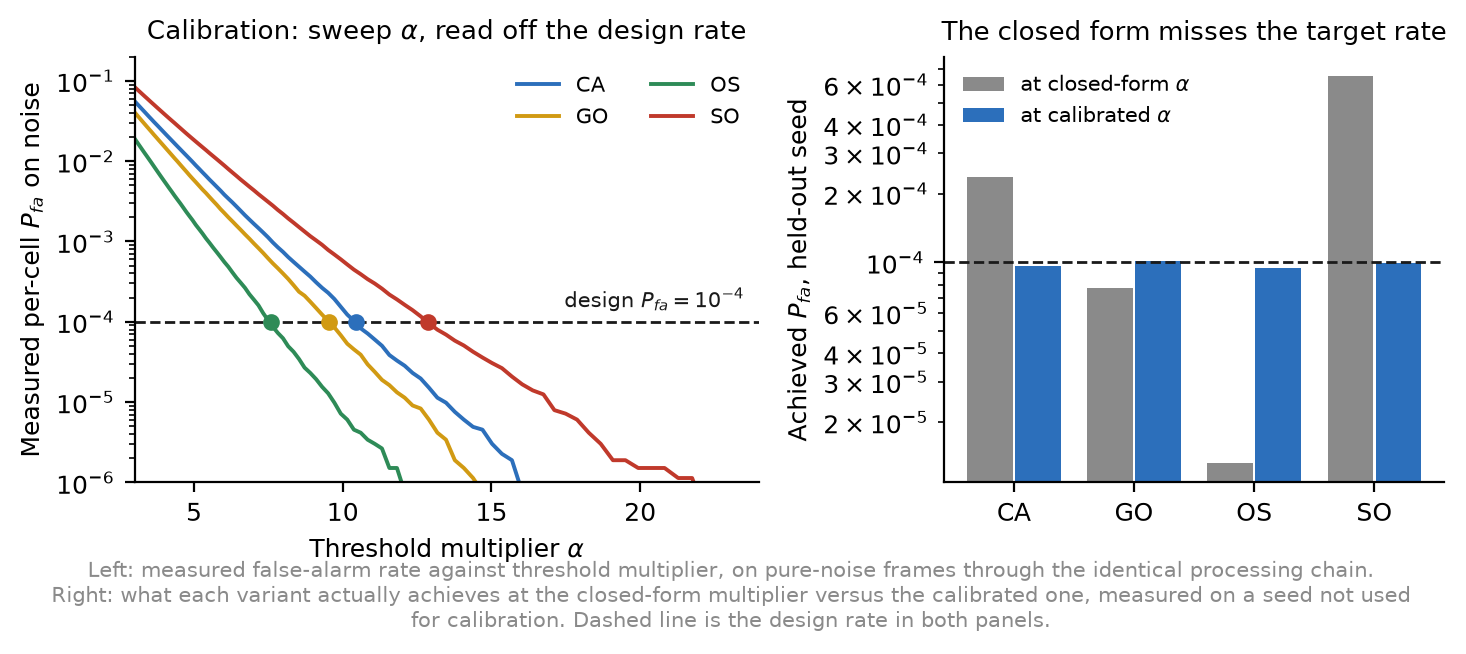
\includegraphics[width=\textwidth]{figures/Chapter4/ch4_fig2_alpha_calibration.png}
\caption[Threshold calibration]{Left: measured false-alarm rate against threshold multiplier for
each variant, on pure-noise frames through the identical chain; the marker is the calibrated value.
Right: the rate each variant achieves at its \emph{analytic reference} multiplier against its
calibrated one, measured on a verification seed not used for calibration. The analytic reference is
defined below and is exact only for CA.}
\label{fig:alphacal}
\end{figure}

The comparison multiplier in the right-hand panel needs defining precisely, because it is not a
set of variant-specific closed forms. It is the CA expression of equation~\eqref{eq:alpha_ca}
applied with the cell count appropriate to each statistic: the full \CfarNRef{} reference cells for
CA and OS, and the half-ring count for GO and SO, which average over half the window. That makes it
\emph{exact for CA}, a reasonable approximation for GO and SO, and, for OS, only a first
approximation --- an order statistic has a different distribution entirely. The figure and
Table~\ref{tab:alphas} therefore label it an \emph{analytic reference}, not a closed-form solution
for each variant.

With that definition, the right-hand panel is the argument. At the analytic reference the achieved
rates are not the design rate: CA overshoots by roughly a factor of two and SO by more than six,
while OS undershoots by nearly an order of magnitude --- the largest error, as expected, for the
variant whose statistic the expression fits worst. After calibration all four sit at the design
rate on data not used to set them.

\begin{table}[H]
\centering
\caption{Calibrated threshold multipliers at a design $\Pfa$ of $10^{-4}$ for the
\CfarWinR{}\,$\times$\,\CfarWinD{} window. The analytic reference is
equation~\eqref{eq:alpha_ca} evaluated with each statistic's cell count; it is exact only for CA.}
\label{tab:alphas}
\begin{tabular}{@{}lccl@{}}
\toprule
\textbf{Variant} & \textbf{Calibrated $\alpha$} & \textbf{Analytic reference} &
\textbf{Status of the reference} \\
\midrule
CA & \CfarAlphaCA & \CfarAlphaCAAnalytic & exact for this statistic \\
GO & \CfarAlphaGO & \CfarAlphaGOAnalytic & half-ring approximation \\
SO & \CfarAlphaSO & \CfarAlphaSOAnalytic & half-ring approximation \\
OS & \CfarAlphaOS & \CfarAlphaOSAnalytic & first approximation only \\
\bottomrule
\end{tabular}
\end{table}

The CA row deserves a comment, since it is the one case where the reference is exact. The
calibrated multiplier is about \SI{10}{\percent} higher, roughly \SI{0.4}{\deci\bel} of extra
threshold. Equation~\eqref{eq:alpha_ca} assumes the \CfarNRef{} reference cells are statistically
independent, whereas the window functions of Chapter~\ref{chp:simulator} correlate neighbouring
cells. The effective number of independent samples is therefore smaller than \CfarNRef{}, and a
higher multiplier is needed to hold the rate.

\textbf{This is not itself a measurement of CFAR loss.} It is a threshold difference on noise-only
data. CFAR loss, as defined in Section~\ref{sec:cfar_loss}, is a \emph{detection} penalty relative
to a detector that knows the true background power. The two are related --- both arise from
estimating the background from finitely many correlated cells --- but they are different
quantities, measured differently, and a value for one is not a value for the other. The
detection penalty is measured separately, against a clairvoyant reference, in
Chapter~\ref{chp:attribution}.

\section{The learned arm}

\subsection{Architecture}

The learned detector, referred to throughout as TinyCNN, is a fully convolutional network that maps
a range--Doppler map to a per-cell score at the same resolution. It has \TinyParams{} parameters.
Figure~\ref{fig:network} shows its structure.

\begin{figure}[H]
\centering
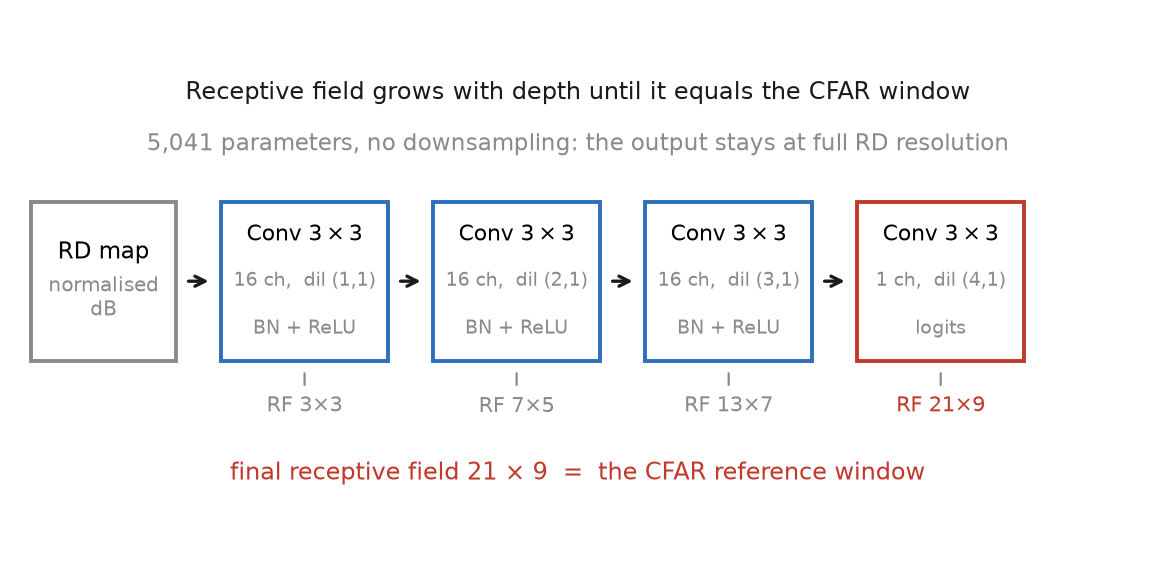
\includegraphics[width=\textwidth]{figures/Chapter4/ch4_fig4_network.png}
\caption[The frozen network]{Four dilated convolutional layers with the receptive field growing to
match the CFAR window. There is no downsampling, so the output remains at full range--Doppler
resolution and no peak is displaced.}
\label{fig:network}
\end{figure}

Three choices define it.

\textbf{The receptive field is matched to the CFAR window.} This is the central design decision of
the project. The layers use dilations $(\TinyDilR)$ along range and $(\TinyDilD)$ along Doppler,
which compose to a receptive field of $\TinyRFR \times \TinyRFD$ --- exactly the window of
Figure~\ref{fig:window}. Dilation is used because it enlarges the receptive field without adding
parameters and without downsampling. The value was verified empirically, by back-propagating from a
single output cell and recording which input cells receive non-zero gradient, rather than trusting
the arithmetic.

\textbf{There is no downsampling.} Padding equals dilation at every layer, so the spatial size is
preserved exactly through the stack. Avoiding a pooling and upsampling stage removes one additional
source of localisation error while keeping the output at full range--Doppler resolution; it does
not by itself guarantee that peaks are placed correctly, which is an empirical question addressed
in Chapter~\ref{chp:synthetic}.

\textbf{The network is deliberately small.} At \TinyParams{} parameters and \TinyWidth{} channels
it is tiny by modern standards. That is intentional: the question is what a small learned local
rule adds over a fixed one, not how well a large network can be made to perform.

\subsection{What ``matched'' does and does not mean}
\label{sec:matched}

The receptive-field match is the fairness argument of this report, so its limits should be stated
plainly.

\textbf{Matching the footprint does not equalise the decision rule.} Both detectors see the same
$\TinyRFR \times \TinyRFD$ neighbourhood, but they use it differently. CFAR takes the cell under
test as its statistic, excludes the guard ring entirely, and estimates the background from the
\CfarNRef{} reference cells. The network has no such partition: all \CfarWinCells{} cells in its
footprint are available to it, and it may combine them in any way its weights encode.

\textbf{This is a structural difference between the two decision rules, not a difference in spatial
footprint.} CFAR excludes the guard cells out of necessity: a simple mean cannot distinguish a
bright neighbour caused by a target's own mainlobe from a bright neighbour caused by high noise. A
learned function is not subject to that constraint. The accurate statement is therefore \emph{the
same footprint, but CFAR is constrained to a hand-derived statistic that requires discarding the
inner cells}. Whether that difference actually contributes to any measured margin is a separate
question, tested in Chapter~\ref{chp:attribution} rather than assumed here.

\textbf{Nominal and effective receptive fields are not the same thing.} It is a general property of
stacked convolutions that influence decays from the centre outward, because central cells
contribute through more paths than edge cells, whereas CFAR weights its reference cells uniformly.
The effective receptive field of this particular network was \emph{not} measured, so this is noted
as an architectural consideration rather than as a measured property of TinyCNN, and no part of the
fairness argument rests on it. The $\TinyRFR \times \TinyRFD$ figure quoted above is the nominal
receptive field, which \emph{was} measured, by back-propagation.

\subsection{Input representation}
\label{sec:inputrep}

The input transform is the highest-leverage preprocessing choice for the learned arm. It is a fixed
part of the detector, applied identically during training and inference: each map is expressed in
decibels relative to \emph{its own frame median power},
\begin{equation}
X = \frac{1}{20}\,\mathrm{clip}\!\left(10 \log_{10}
\frac{P}{\operatorname{median}(P)},\; -10,\; +60\right),
\label{eq:norm}
\end{equation}
where $P$ is the range--Doppler power map.

The frame median is used as the reference level rather than the frame maximum. Peak normalisation
would rescale every frame by its brightest target and destroy the absolute signal-to-noise
information the detector needs. The median is a robust measure of the frame's background scale: in
the homogeneous synthetic frames of Chapter~\ref{chp:simulator} it tracks the noise level closely,
but it is a statistic of the frame, not a measurement of physical noise power, and the two need not
coincide in cluttered scenes or in real data. Chapter~\ref{chp:realdata} returns to this point,
since the same fixed transform must then be applied to frames whose background statistics differ
from those it was fitted on.

As noted in Section~\ref{sec:whatiscommon}, this transform has no counterpart in the classical arm,
which works from power directly. That is a real difference between the two paths, and it is part of
what each detector is rather than an adjustable knob.

\subsection{Labels}
\label{sec:labels}

Section~\ref{sec:sota} noted that a learned detector must be given a training target and that the
choice is not neutral. The label used here is a $3\times3$ block centred on each target's cell.

A block label asks the network to respond over a small region rather than at one exact cell, which
relaxes the localisation demand relative to a single-cell label. It is retained here because it
belongs to the frozen benchmark: changing it would mean the reported results no longer describe the
system that produced them.

Its effect is not left as an open question. Chapter~\ref{chp:attribution} tests the label
representation explicitly, training under alternative supervision while leaving the frozen
benchmark intact, so that the influence of this choice on localisation is measured rather than
assumed.

\subsection{Training}

Table~\ref{tab:training} gives the training configuration. Every entry is a recorded choice rather
than a default, and the whole configuration was frozen before any benchmark split was scored. It
was not revisited afterwards: the one later protocol change described in
Appendix~\ref{app:prereg} touches candidate extraction, not the network or its training.

\begin{table}[H]
\centering
\caption{Frozen training configuration. Read from the frozen contract when this report is built.}
\label{tab:training}
\begin{tabular}{@{}lll@{}}
\toprule
\textbf{Setting} & \textbf{Value} & \textbf{Note} \\
\midrule
Loss & \texttt{BCEWithLogits} & with positive-class weighting \\
Positive weight & \TinyPosWeight & chosen by ablation, not class balancing \\
Optimiser & Adam & learning rate \TinyLR, batch \TinyBatch \\
Epochs & \TinyEpochs & pre-registered selection rule, below \\
Early stopping & off & deliberately \\
Seeds & \TinySeeds & all reported; single-seed results not trusted \\
Threads & \TinyThreads & load-bearing, see below \\
Training split & \texttt{bench2\_train} & \BenchTrainFrames{} frames \\
Selection split & \texttt{bench2\_val} & \BenchValFrames{} frames \\
\bottomrule
\end{tabular}
\end{table}

Three of those entries need explanation.

\textbf{Epoch selection.} The reported epoch was not chosen by early stopping, because validation
loss plateaus later than detection probability does and would select the wrong epoch. The procedure
was instead:
\begin{enumerate}
\itemsep1pt
\item every epoch from 1 to 25 was evaluated on the validation split;
\item detection probability was pooled over the \TinySeeds{} seeds at each epoch;
\item the selected epoch is the \emph{earliest} whose pooled value lies within one standard error
of the plateau.
\end{enumerate}
The rule was fixed before the sweep was examined. It is described here as pre-specified rather than
pre-registered: it was written down in advance, but not lodged as a formal pre-registration in the
way the real-data protocol of Chapter~\ref{chp:realdata} was.

\textbf{Positive weighting.} The positive class is vastly outnumbered, and exact class balancing
would imply a weight near 974. That value was tried and produced a result that later had to be
retracted; the weight of \TinyPosWeight{} won a three-way ablation on the validation split. The
retraction is recorded in Appendix~\ref{app:corrections}.

\textbf{Thread count is load-bearing.} CPU tensor kernels accumulate in a different order at
different thread counts, so the same seed trained with a different thread count produces different
weights. The count is fixed at \TinyThreads{} as part of the reproducibility contract, not as a
performance setting, and runs trained at different thread counts are not pooled or compared. The
measured size of the effect is recorded in Appendix~\ref{app:tables}.

\textbf{Eight seeds are reported, always.} A single training run is one sample from a distribution,
and the spread between seeds is not negligible. Every network result in this report is a mean over
\TinySeeds{} seeds with the individual seeds shown.

\section{The evaluation protocol}

\subsection{One rulebook}

Each detector produces its own score map. CFAR works from linear power and produces a ratio map.
The network applies the normalisation of Section~\ref{sec:inputrep} and produces a logit map.

Everything after that point is shared. Both maps go through the same code, in the same order:
\begin{center}
score map $\rightarrow$ peak extraction (NMS) $\rightarrow$ operating threshold\\[2pt]
$\rightarrow$ one-to-one matching $\rightarrow$ metrics
\end{center}

\begin{figure}[H]
\centering
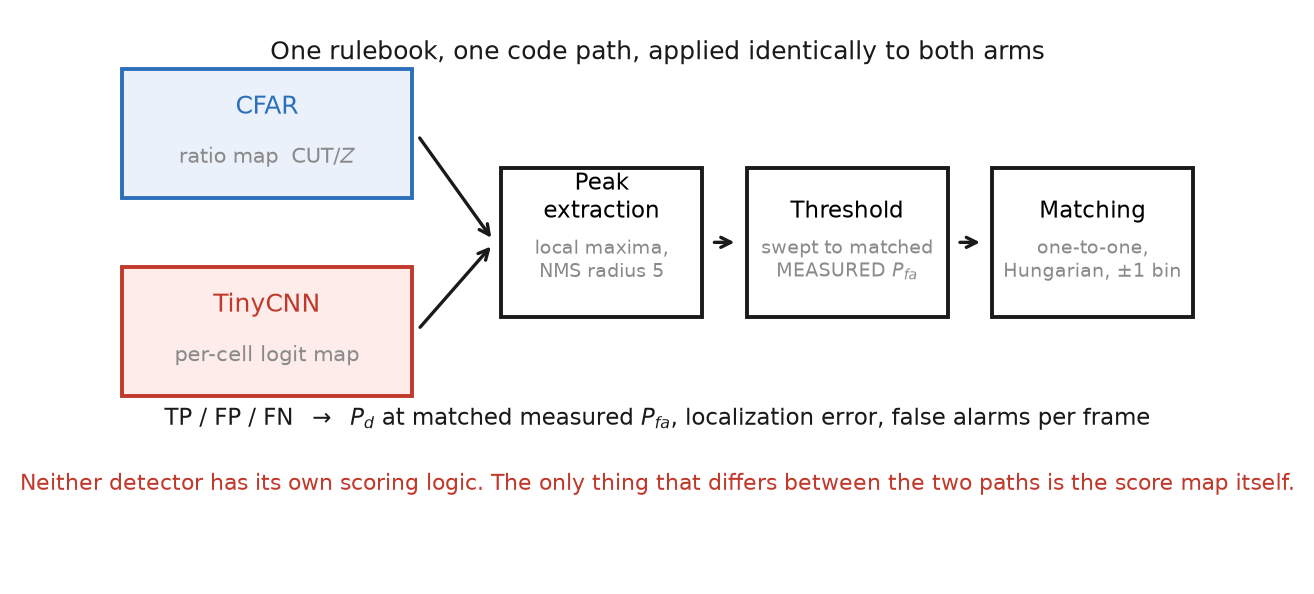
\includegraphics[width=\textwidth]{figures/Chapter4/ch4_fig5_protocol.png}
\caption[The shared evaluation protocol]{Both arms are reduced to point lists and scored through a
single code path. What differs between the two routes is the score map and the fixed
detector-specific transform that produces it; everything downstream --- candidate extraction,
thresholding, matching and scoring --- is shared.}
\label{fig:protocol}
\end{figure}

\subsubsection*{Peak extraction}

A strong target does not produce one bright cell. It produces a small cluster of bright cells, and
several of them may be local maxima. Non-maximum suppression (NMS) reduces each cluster to its
strongest cell.

A cell is kept as a candidate if it is the largest value in its neighbourhood. The neighbourhood is
a square set by a suppression radius $r$,
\begin{equation}
\text{side} = 2r + 1 ,
\label{eq:nmsside}
\end{equation}
so $r = 1$ gives $3 \times 3$, $r = 2$ gives $5 \times 5$, $r = 3$ gives $7 \times 7$ and $r = 5$
gives $11 \times 11$. This protocol uses $r = \ProtocolNms$, a
$\ProtocolNmsWin \times \ProtocolNmsWin$ window.

Candidates are extracted \emph{before} any threshold is applied. The candidate set is therefore
computed once and reused at every threshold the score sweep visits.

\subsubsection*{Selecting the suppression radius}
\label{sec:nmschoice}

The radius is a post-processing constant, not a property of either detector. It was chosen on
development data only: the tuning split for selection, the validation split for confirmation.
Neither the held-out benchmark of Chapter~\ref{chp:synthetic} nor any real data of
Chapter~\ref{chp:realdata} contributed to the choice.

Radii \NmsRadiiTested{} were compared at matched measured $\Pfa$, with the threshold re-derived at
each radius so that a drifting false-alarm rate could not confound the comparison.
Figure~\ref{fig:nmssel} shows the four panels that decide it.

\begin{figure}[H]
\centering
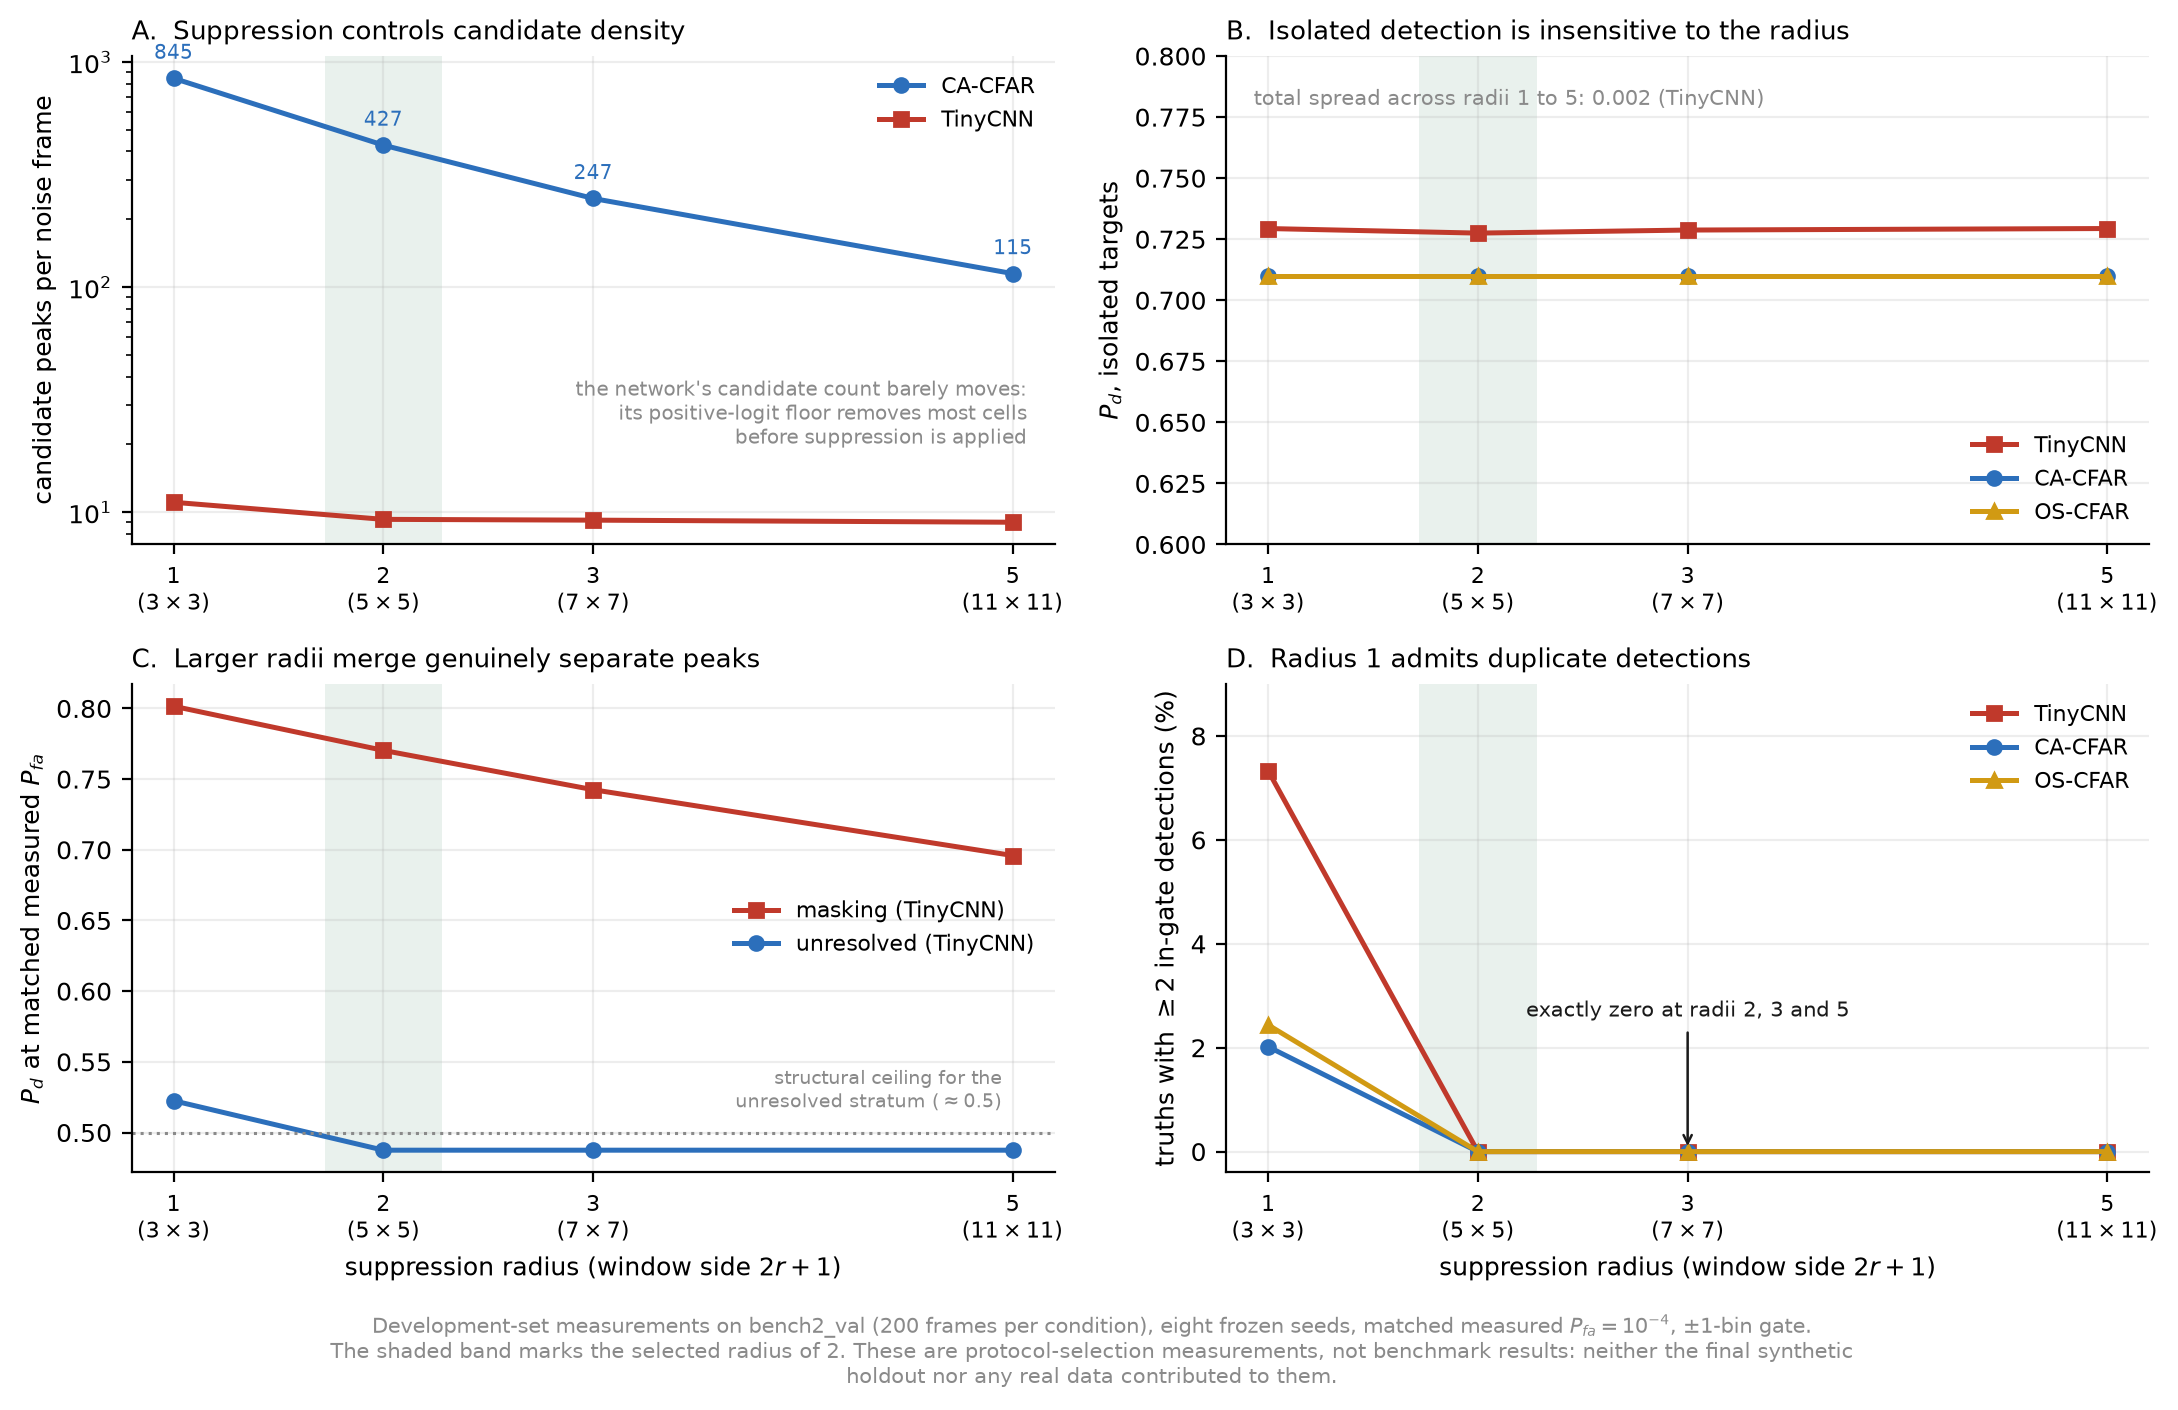
\includegraphics[width=\textwidth]{figures/Chapter4/ch4_fig8_nms_selection.png}
\caption[Selecting the non-maximum-suppression radius]{Selection of the suppression radius, on
\textbf{development data only}. \textbf{A}: candidate density on pure-noise frames, the quantity
the radius directly controls. \textbf{B}: detection probability on isolated targets, which is
essentially flat across radii. \textbf{C}: the masking and unresolved strata, where a larger window
merges peaks belonging to different targets. \textbf{D}: the fraction of truths receiving two or
more detections inside their gate, which is non-zero only at radius~1. Shading marks the selected
radius. \textbf{These are protocol-selection measurements, not benchmark results}: the final
synthetic holdout of Chapter~\ref{chp:synthetic} and the real data of
Chapter~\ref{chp:realdata} were not used, and no real-data information of any kind entered this
choice.}
\label{fig:nmssel}
\end{figure}

\textbf{Panel A: a smaller radius keeps more candidates.} Going from $r = 5$ to $r = 1$ raises
CA-CFAR's candidate count on noise frames from \NmsCandFive{} to \NmsCandOne{} per frame, a factor
of \NmsCandRatio{}. The network's count barely moves, because its positive-score floor already
removes most cells before suppression runs.

\textbf{Panel B: that extra density costs almost nothing in detection.} One might expect the extra
candidates to force a higher threshold at fixed measured $\Pfa$, and so lose weak targets. They do
not. Isolated-target $\Pd$ varies by less than \NmsIsolatedSpread{} across the whole range, for
every arm. Suppression sets how densely candidates are spaced; the threshold sets how strong they
must be. On this benchmark the first does not translate into lost detections.

\textbf{Panel C: a large radius merges nearby real targets.} This is the real cost. On the masking
stratum the network's $\Pd$ falls steadily as the window grows, from \NmsMaskingOne{} at $r = 1$ to
\NmsMaskingFive{} at $r = 5$. A window of side $\ProtocolNmsOriginalWin$ is far wider than the
measured point-target mainlobe of Chapter~\ref{chp:simulator}, so it removes genuine responses from
neighbouring targets, not just noise.

\textbf{Panel D: at $r = 1$ one target can produce two counted detections.} Several peaks from a
single response survive suppression, and Section~\ref{sec:matching} explains how they can then be
credited to two different truths. Between \NmsDupOneMin{} and \NmsDupOneMax{} of the network's
matched truths receive a second in-gate detection at $r = 1$, and up to \NmsDupOneCFAR{} of
CA-CFAR's, against \NmsDupOther{} at every larger radius.

The unresolved stratum makes that visible. It places two targets close enough that they cannot be
resolved cleanly, so roughly one response is expected for two truths and $\Pd$ near $0.5$ is the
intended outcome. At $r = 1$ the measured value is \NmsUnresolvedOne{}, and every arm shows the
same lift. This is treated as evidence, not as proof: $0.5$ is what the construction is designed to
produce, not a mathematical limit. What makes it diagnostic is that the lift appears only at the
radius that also produces duplicate detections, and in exactly the direction that mechanism
predicts.

\textbf{Radius \ProtocolNms{} was selected because it was the smallest tested radius that removed
duplicate detections while preserving close-target separation.} That is a statement about this
evaluator on this benchmark, not a claim of a universal optimum.

One limitation remains. A $\ProtocolNmsWin \times \ProtocolNmsWin$ window is still wider than a
single point-target mainlobe, so it bounds how close two targets can be and still be reported
separately. Chapter~\ref{chp:realdata} returns to this, because real annotated objects are
\emph{larger} than the suppression window --- a regime the synthetic benchmark never exercises.

\subsubsection*{The valid region}

CFAR cannot form its full $\CfarWinR \times \CfarWinD$ window near the border, so the outer margin
is excluded: $\CfarGuardR + \CfarTrainR = 10$ bins on the range axis and
$\CfarGuardD + \CfarTrainD = 4$ on Doppler.

The same mask is applied to the network. Both detectors are therefore scored on exactly the same
cells, and the false-alarm denominator counts the same cells for both.

\begin{figure}[H]
\centering
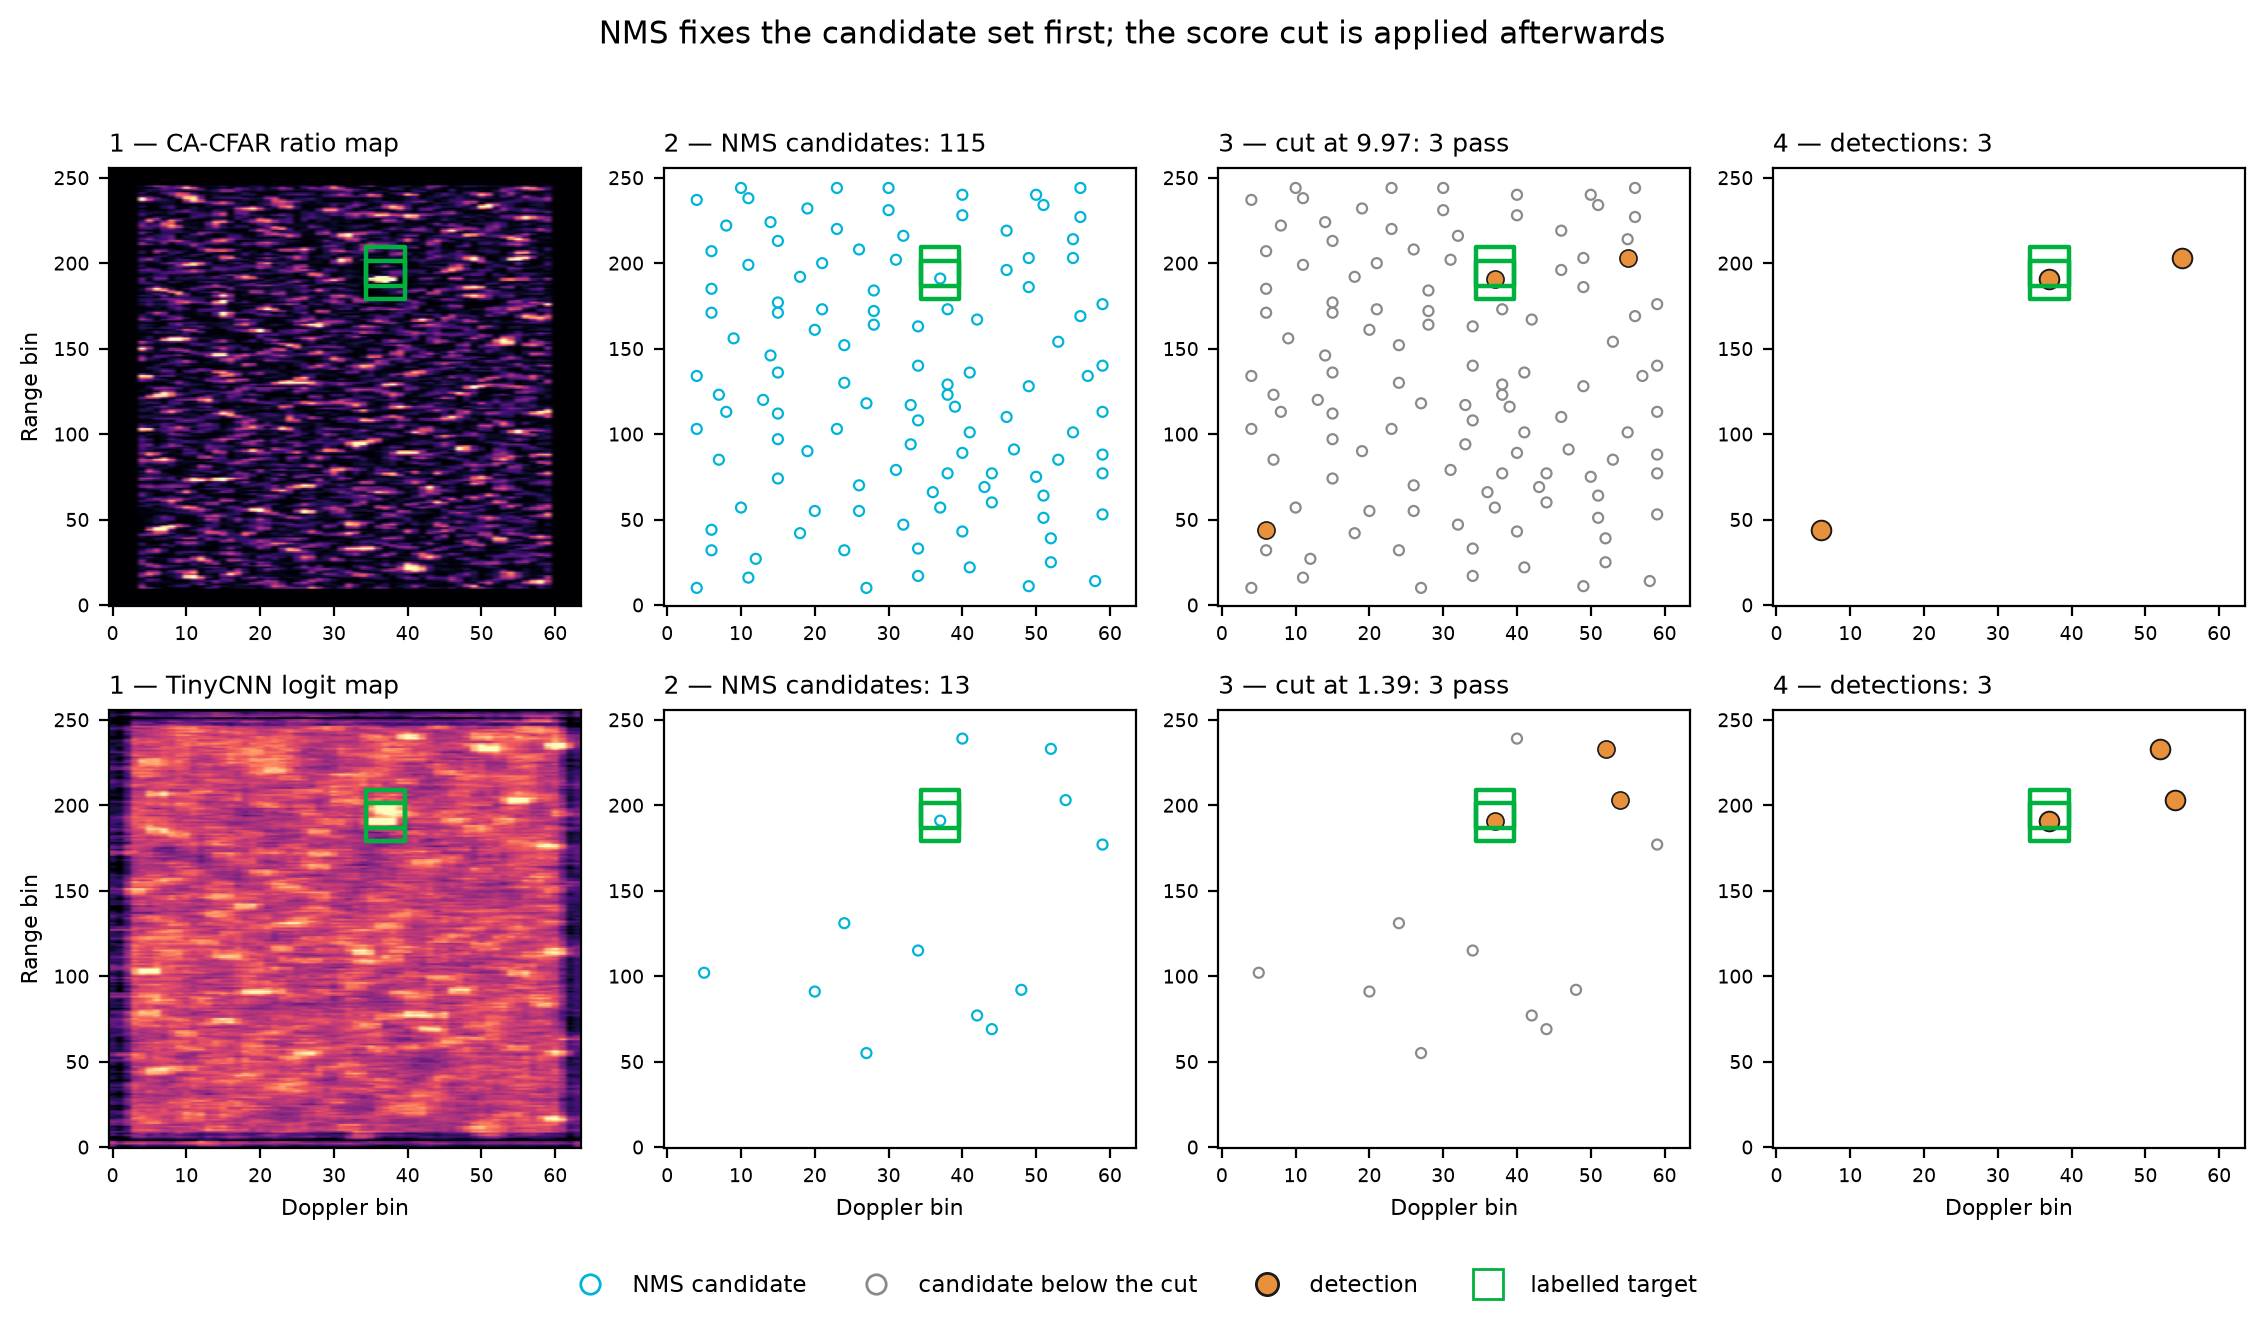
\includegraphics[width=\textwidth]{figures/Chapter4/ch4_fig6_pipeline_stages.png}
\caption[The four evaluation stages on one frame]{The shared pipeline executed on a single
\texttt{masking} frame from the validation split, for CA-CFAR (top) and the network (bottom).
Stage~2 fixes the candidate set; stage~3 then applies the score cut to those candidates.
\textbf{This is an illustrative frame, not a benchmark result.} The two arms reach the same
detection count from very differently shaped score maps: CFAR's above-threshold cells are already
nearly isolated, whereas the network responds with a broader region that suppression must collapse.
The numerical cuts shown are the matched values for \emph{this} condition and frame, and are not
universal deployment thresholds.}
\label{fig:stages}
\end{figure}

\subsubsection*{The candidate score floor}

The shared extractor keeps only cells with a strictly positive score. CFAR scores are ratios of
powers and are always positive, so nothing is removed. Network scores are logits, which are
negative wherever the predicted probability is below one half, so those cells can never become
candidates.

This does not affect any reported result: the operating points used here lie well above zero. It
does truncate the extreme high-$\Pfa$ tail of the network's ROC curve, which cannot extend below a
logit of zero. ROC comparisons in that far tail should be read with the asymmetry in mind.

\subsection{Matching}
\label{sec:matching}

A detection matches a truth if it lies inside the tolerance gate,
\begin{equation}
|\Delta r| \le G_r \quad\text{and}\quad |\Delta v| \le G_v .
\end{equation}

Matching is one-to-one, computed by Hungarian assignment on the distance between candidate and
truth. Hungarian assignment chooses the pairing that minimises total distance, with pairs outside
the gate made unaffordable. A matched detection is a true positive; an unmatched truth is a false
negative.

Two consequences follow for detections that land near a real target.

\begin{itemize}
\itemsep2pt
\item \textbf{One truth gives at most one true positive.} If several detections fall inside one
isolated target's gate, exactly one is matched and the rest are ignored --- neither credited nor
charged as false alarms. Cells inside a truth's gate also leave the false-alarm denominator, so the
detector is not credited for correctly rejecting them either.
\item \textbf{Two nearby truths are different.} If their gates overlap, or one physical response
spans both, the assignment may give one peak to each truth. Several peaks from a \emph{single}
response can then be counted as \emph{two} detections. Since surplus in-gate detections cost
nothing, a detector that emits many close peaks gets extra attempts for free.
\end{itemize}

That second case is the free-attempt behaviour the suppression sweep found at $r = 1$, and it is
why the radius was not chosen on detection probability alone. The rule is applied identically to
both arms.

\begin{figure}[H]
\centering
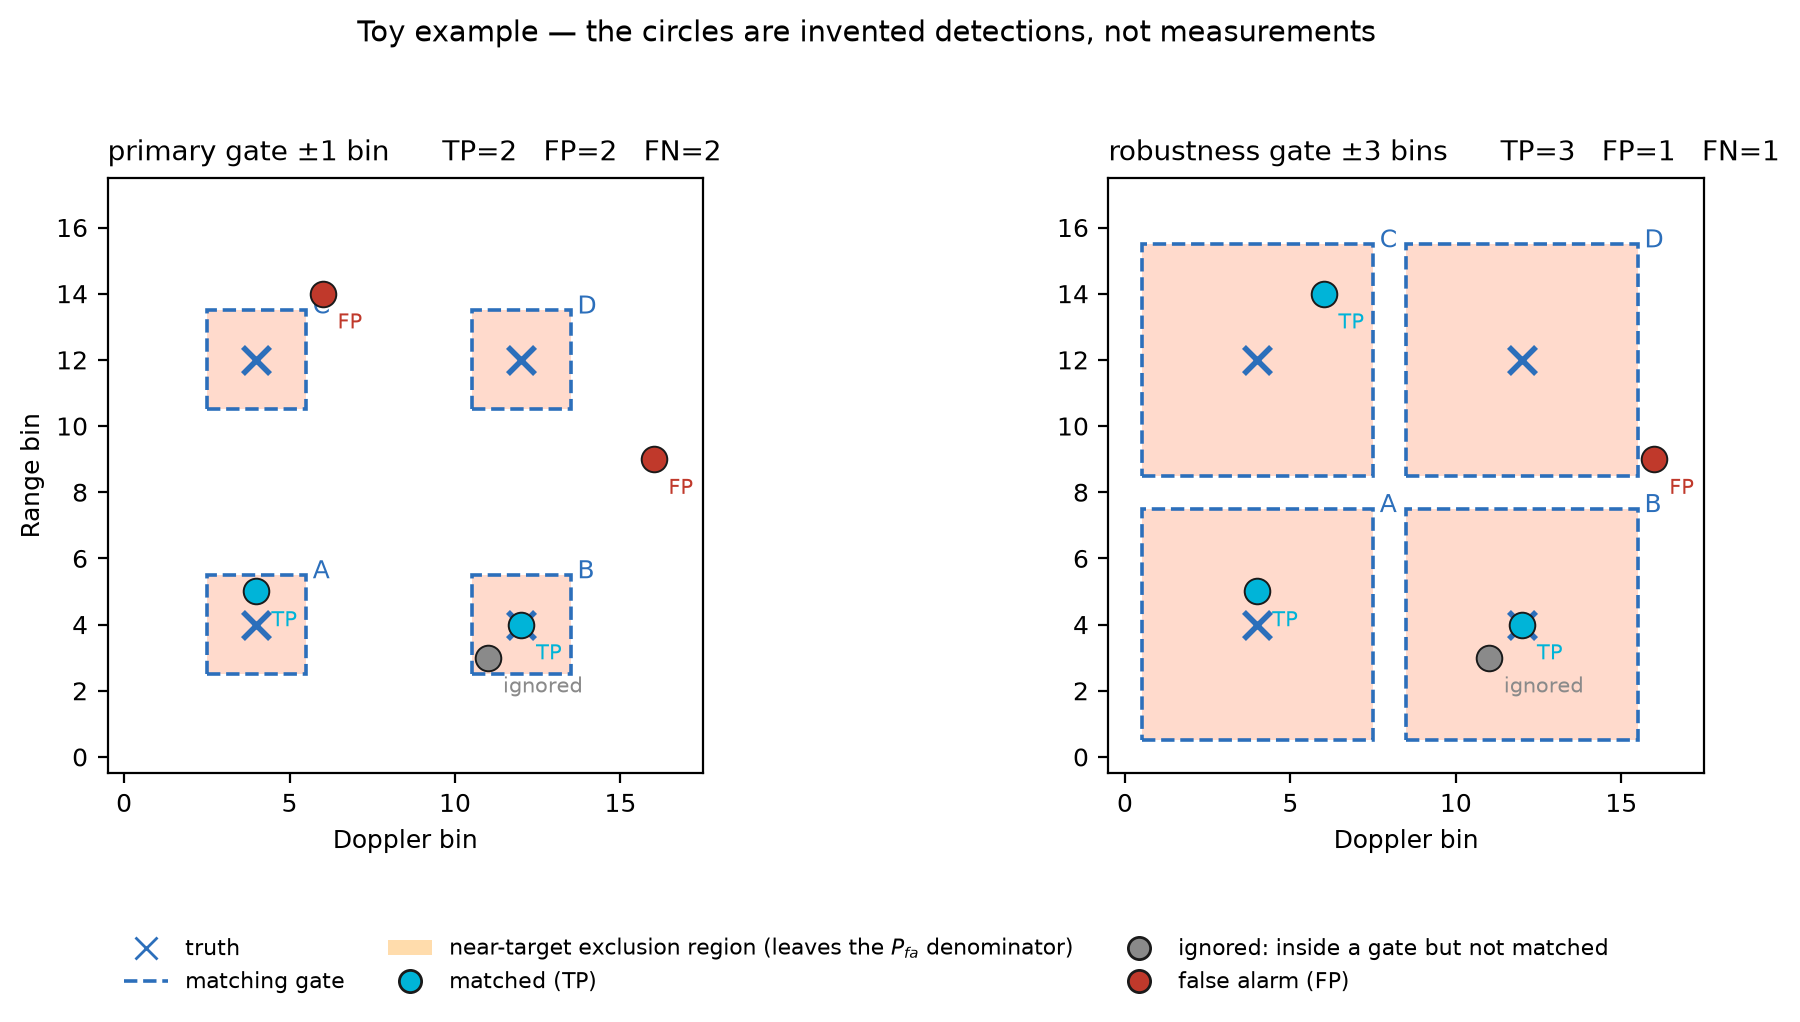
\includegraphics[width=\textwidth]{figures/Chapter4/ch4_fig7_matching.png}
\caption[Matching and tolerance on a worked example]{A toy frame with four truths and five
detections, scored by the same function used throughout this report. \textbf{The detections are
invented to exercise every outcome; they are not measurements.} Left, the primary
$\pm\ProtocolGate$-bin gate: A and B are matched, the second detection near B is ignored because B
is already taken, the detection two bins from C falls outside the gate and so is both a miss and a
false alarm, and D is a plain miss. Right, the same frame at $\pm\ProtocolGateRobust$ bins: the
detection near C now falls inside its gate and becomes a match, which is precisely what the wider
tolerance is reported to reveal.

The shaded area is the near-target exclusion region, drawn from the matching gate. \textbf{It is
not the CFAR guard region of Figure~\ref{fig:window}}, which is a different construct serving a
different purpose, as explained below.}
\label{fig:matching}
\end{figure}

Two shaded regions appear in this chapter and they are easy to confuse. The \textbf{CFAR guard
cells} of Figure~\ref{fig:window} belong to the detector: they keep a target's own energy out of
the background estimate. The \textbf{near-target exclusion region} of Figure~\ref{fig:matching}
belongs to the evaluator: it decides which unmatched detections count as near misses rather than
false alarms. One is built from the CFAR window geometry, the other from the matching tolerance,
and they need not have the same extent.

\subsection{Operating point}
\label{sec:opoint}

The headline synthetic comparison is $\Pd$ at matched \emph{measured} $\Pfa$. Each detector's score
threshold is swept, the achieved false-alarm rate is measured at each setting, and the two arms are
compared where those achieved rates agree.

This is stricter than matching at design $\Pfa$. Figure~\ref{fig:alphacal} showed that achieved and
design rates differ, and by different amounts for different variants, so matching on the achieved
rate removes that confound.

The sweep is performed \emph{per condition}. Each stratum gets its own sweep, and the arms are
compared at the same measured false-alarm level within that stratum. This is an \textbf{evaluation
operating point, not a deployable threshold}: it requires labels on the data being scored, and one
global setting would not achieve the same rate in every condition.

Chapter~\ref{chp:realdata} works differently, and the contrast matters. There the network must run
at a single fixed threshold derived from synthetic validation data alone, without access to the
real data it is scored on. That is a harder requirement than the per-condition matching used here.

\subsection{Tolerance}

The primary gate is $\pm\ProtocolGate$ bin, fixed in advance. A gate of $\pm\ProtocolGateRobust$
bins is reported beside it as a robustness check, never instead of it.

Reporting both separates detection from localisation. A detector that finds a target but places it
two bins away is credited at the wider gate and not at the narrower one --- the detection near
truth~C in Figure~\ref{fig:matching}. Comparing the two numbers therefore shows how far a
conclusion depends on localisation tolerance. Both are reported for every condition, whichever way
they point.

\subsection{Statistics}

Differences are assessed by a paired bootstrap with \ProtocolBootstrap{} resamples. \textbf{The
resampling unit is the frame.} Frames are drawn with replacement, and within each resample both
arms are re-scored on exactly the same frames, so frame difficulty cancels instead of adding noise.
Resampling whole frames also preserves the dependence among targets belonging to the same frame.

Seven conditions are scored, so significance uses a Bonferroni correction: a per-condition
threshold of $\alpha = \ProtocolBonf$ against a family-wise $0.05$.

One limitation should be noted. The operating threshold is computed once per condition and held
fixed across resamples, so the intervals capture sampling error in $\Pd$ at a fixed operating
point. They do not include the uncertainty in choosing that threshold, which would require redoing
the sweep inside every resample. The reported intervals are therefore slightly optimistic.

\subsection*{Summary of the protocol}

Both detectors see comparable $\CfarWinR \times \CfarWinD$ local context and generate their score
maps by their own fixed transforms. Everything downstream is identical: NMS at radius
\ProtocolNms{}, a threshold set to match \emph{measured} $\Pfa$ per condition, one-to-one Hungarian
matching, and metrics from a single code path. Results are reported at the
$\pm\ProtocolGate$-bin gate and at the $\pm\ProtocolGateRobust$-bin robustness gate, with paired
frame bootstraps and a Bonferroni correction across the seven conditions.

\section{Conclusion}

Both detectors are now fully specified, and so is the instrument that will measure them.

The classical arm uses a \CfarWinR{}\,$\times$\,\CfarWinD{} window whose guard count follows the
measured point spread function and whose shape was selected on a split reserved for that purpose,
with SO the one variant that did not take part in that selection. Its four multipliers are
calibrated on noise-only data rather than taken from an analytic expression which, as measured
here, does not deliver the design false-alarm rate for any of them.

The learned arm is a \TinyParams{}-parameter fully convolutional network whose receptive field
composes to the CFAR window. The limits of that match are set out in Section~\ref{sec:matched}: the
arms share a spatial footprint, not a decision rule, and the network is not obliged to discard the
guard cells that CFAR must exclude. Whether that difference matters is left to
Chapter~\ref{chp:attribution} to test.

What the two arms hold in common, and where they differ, is stated in
Section~\ref{sec:whatiscommon}: the same frames, a comparable footprint and one shared evaluation
path, but each with its own fixed input transform. The protocol reduces both to point lists and
scores them through a single code path at matched measured false-alarm rate, at two tolerances,
with paired frame bootstrap intervals and a correction for multiple comparisons. Its two known
asymmetries --- the positive-score candidate floor, and the fact that the operating point is an
evaluation construct rather than a deployable threshold --- are recorded above rather than left for
a reader to find.

The protocol was fixed, and the network configuration frozen, before the test split was read.

Chapter~\ref{chp:synthetic} now reports what that measurement returned.
